\documentclass{article}

\usepackage{graphicx}
\usepackage{hyperref}
\usepackage{float}
\usepackage{enumitem}
\usepackage{pdfpages}
\usepackage{caption}

\title
{
	Practica 3\\
	Algoritmos de Ordenamiento Parte 3
}

\author
{
	Román Jimenez Adolfo
}

\begin{document}
	
	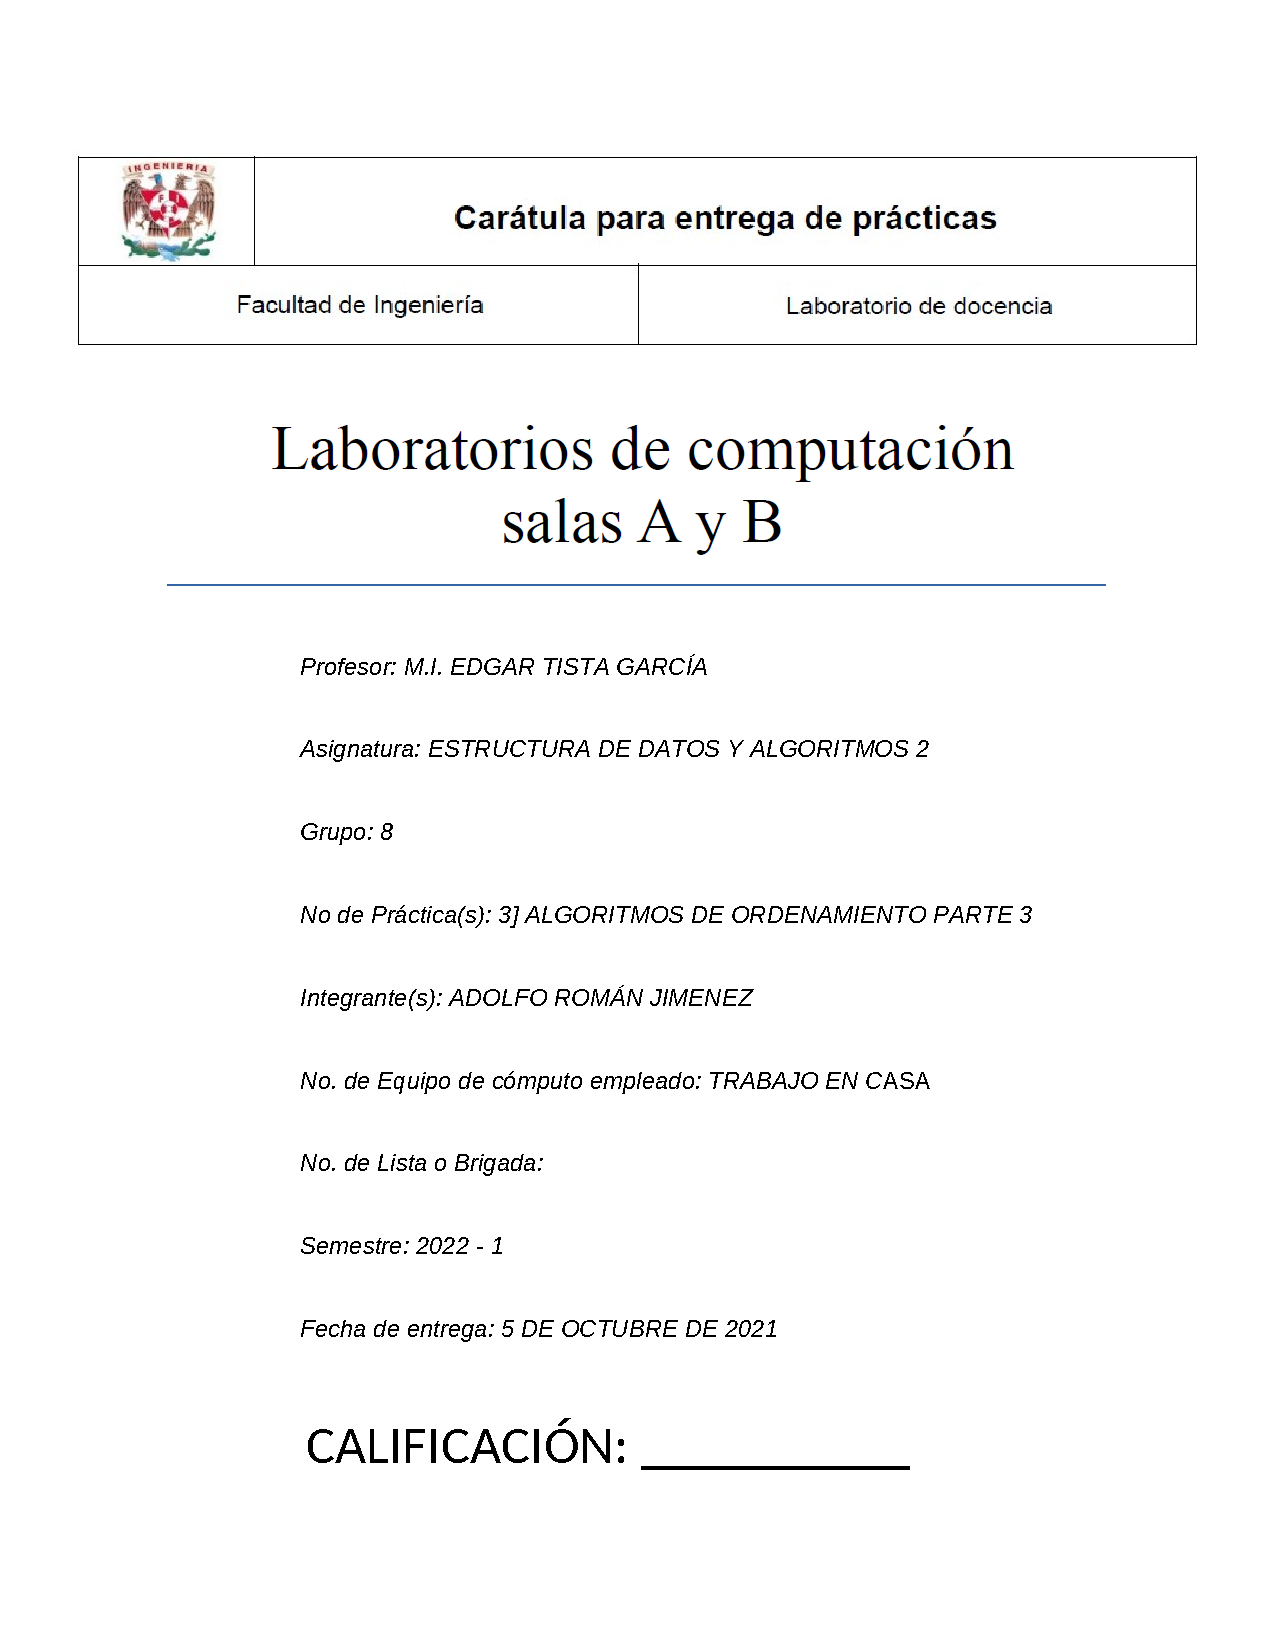
\includepdf[pages=-]{p3car.pdf}
	
	\maketitle
	
	\section{Objetivo}
		
		El estudiante identificará la estructura de los algoritmos de ordenamiento Counting Sort y Radix-sort
	
	\section{Objetivo de Clase}
		
		El alumno implementará casos particulares de estos algoritmos para entender mejor su funcionamiento a nivel algorítmico.
		
	\newpage
		
	\section{Desarrollo}
		\subsection{Ejercicio 0: Menu y Auxiliares}
		
			El menu creado para el Ejercicio 0, es un menu sencillo que solamente incluye las opciones de los algoritmos de ordenamiento a que la practica solicita.\\
			
			El menu contiene las opciones:
			
			\begin{itemize}
				\item Counting Sort
				\item Radix
				\item Exit
			\end{itemize}
			
			Este menu esta contenido dentro del archivo \verb|options.c| bajo la funcion \emph{menu} y contiene como argumento un apuntador que almacenara la informacion obtenida por el usuario en una variable entera externa \textbf{option} para escoger la opcion solicitada por el usuario al momento de probar el algoritmo deseado.\\
			
			El menu esta contenido dentro de un \emph{while-loop} que rompe el ciclo hasta que el usuario escoge una de las 3 opciones numericas validas, mientras no lo haga, este seguira ejecutandose.\\
			
			Al momento de escoger una opcion valida, esta se almacena dentro de una variable interna \textbf{n} que despues se deposita dentro del apuntador.
			
			\begin{figure}[H]
				\centering
				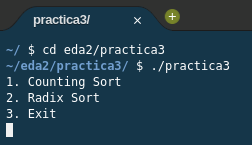
\includegraphics[scale = 1]{images/m1.png}
				\caption*{Ejercicio 0: Menu}
			\end{figure} 
			
		\newpage
			
		\subsection{Ejercicio 1: Counting Sort}
		
			Para programar el algoritmo de ordenamiento \emph{CountingSort()} me base directamente en el pseudocodigo contenido dentro del video de la clase y lo trate de transcribir de la mejor forma posible a como ahi se mostraba, aunque tuve que agregar algunos detalles para que mi codigo funcionara de forma mas eficiente.\\
			
			El algoritmo de \emph{CountingSort()}, se encuentra dentro del archivo \verb|counting.c| y consta de 4 funciones que estan ordenadas en forma descendente a como aparecen en la siguiente lista:
			
			\begin{itemize}
				\item \emph{findMax()}
				\item \emph{fillZeros()}
				\item \emph{restore()}
				\item \emph{countingSort()}
			\end{itemize}
		
			De forma general, \emph{CountingSort()} obtiene el arreglo a ordenar y utiliza la funcion \emph{findMax()} para iterar dentro de este arreglo y obtener el valor mayor del arreglo. Despues, crea un arreglo de la longitud de ese valor maximo y utiliza \emph{fillZeros()} para igualar todas las posiciones dentro del arreglo creado a 0's. Acto seguido, el programa itera sobre el arreglo originar para contabilizar el numero de veces que se repiten los elementos en este y registrar ese numero de veces dentro del nuevo arreglo creado, para despues sumar los elementos de este arreglo de forma recursiva conforme a cada una de las casillas del arreglo y por ultimo usa la funcion \emph{restore()} para reescribir los elementos ordenados en un nuevo arreglo previamente creado.\\
			
			A continuacion se ofrece una explicacion mas detallada sobre el funcionamiento de cada una de las funciones del algoritmo por orden de uso. 
		
			\subsubsection{optionOne()}
			
				Despues de que se escoge la opcion deseada, dentro de la funcion \emph{main()} el codigo se dirige hace un operador ternario que evalua el valor de \textbf{option} y cuando el valor es 1, entonces se dirige a ejecutar la funcion \emph{optionOne()}.\\
				
				La funcion \emph{optionOne()} esta contenida dentro del archivo \verb|options.c| y es la que proporciona todos las variables necesarias a \emph{countingSort()} para operar.\\
				
				Como el ejercicio solicita que \emph{CountingSort} opere con una arreglo de 20 elementos, primeramente se declara una variable de tipo entero y se le asigna un valor de 20 que es el número de elementos que el ejercicio recomienda para la práctica. Acto seguido, se declaran dos arreglos de caracteres estos y estos arreglos tendrán el tamaño de la variable size, por lo que podrán almacenar un máximo de 20 caracteres cada uno.\\ 
				
				El primer arreglo lleva por nombre \textbf{arr} en este arreglo se ingresarán os caracteres que se pretende ordenar, el segundo arreglo lleva por nombre \textbf{sorted} y es dentro de este arreglo donde se escribirán los caracteres ya ordenados.\\
				
				Después de esto se invoca a la función \emph{charGet()} que toma dos argumentos. El primero un arreglo de caracteres y el segundo, una variable de tipo entero. La función \emph{charGet()} primeramente imprime una leyenda que invita al usuario a ingresar los 20 caracteres que pretende ordenar. Después de esto se declara una variable de tipo \textbf{char} y acto seguido se activa un \emph{for-loop} el cual comienza en 0 y termina hasta que itera hasta la ultima posicion del indice que es menor a 20. El \emph{for-loop} utiliza la función \emph{getChar()} que deposita en la variable \textbf{a} y despues evalúa si la variable no incluye un salto de línea; si lo incluye, entonces de se deshace del salto de línea y pasa al siguiente elemento que finalmente deposita la variable contenida en el indice correspondiente al arreglo.\\
				
				Cuándo la funcion alcanza un total de 20 iteraciones finaliza su ejecución.\\
				
				Después de esto se utiliza una función para imprimir el arreglo de la cual hablaremos después y se procede a ingresar a la funcion del algoritmo \emph{countingSort()}.
			
			\subsubsection{countingSort()}
			
				El algoritmo \emph{countingSort()} usa tres argumentos los cuales son: el arreglo de caracteres donde se encuentran los elementos en desorden, una variable de tipo entero que contiene la longitud del arreglo y otro arreglo de caracteres que es dónde se ordenarán los elementos.\\
				
				La función comienza declarando un arreglo de dos enteros que servirá para depositar el valor minimo y maximo, el cual constituria el rango de los elementos del arreglo. Asimismo, declara una variable de tipo entero \textbf{elem} qué después funcionara como una variable auxiliar.\\ 
				
				Después de esto, el programa invoca a la función \emph{findMax()} y cuando está finaliza ya se encuentran depositados en el arreglo auxiliar, dentro de el índice 0, el rango y en el índice 1, el valor mínimo en el  arreglo.\\
				
				Después de esto se declara otro arreglo de tipo entero \textbf{count} y qué tiene posee una longitud del valor contenido en la variable \textbf{max} la cual representa el total rango entre los elementos mínimo y máximo del arreglo original que pretendemos ordenar.\\
				
				Dado esto se procede a llenar con ceros las posiciones del nuevo arreglo por medio de la funcion \emph{fillZeros()} para su uso posterior.\\
				
				Una vez que el arreglo ha sido llenado con ceros, se declara un \emph{for-loop} que iterara desde el número 0 hasta 1 antes de llegar al tamaño del arreglo, esto quiere decir que sus ciclos iran desde el indice 0 hasta el 19 qué son los índices donde se contienen los caracteres de el arreglo que pretendemos ordenar. Ya dentro de este \emph{for-loop} se toma cada uno de los caracteres en \textbf{arr} y se les hace un \emph{casting} a tipo entero que convierte su valor a codigo \verb|ASCII|.\\
				
				Después se resta ese valor en código \verb|ASCII| al valor contenido en \textbf{min} y esto da como resultado el índice al que el elemento corresponde dentro del arreglo \textbf{count} por lo que se procede a sumar 1 a ese índice y es de esta forma cómo se registra que la frecuencia los caracteres existentes dentro en el arreglo a ordenar. Esto se hace con todos los demás elementos y asi se obtiene una “lista” de los elementos existentes y su frecuencia.\\
				
				Cuando este proceso termina Se imprime el arreglo.\\
				
				Después de esto se procede a iterar dentro de los elementos del arreglo \textbf{count}; se comienza desde el índice número 1 hasta 1  antes del valor en \textbf{max}, no hay que olvidar que el valor en \textbf{max} corresponde al rango de los elementos, por lo que esto es igual a la longitud del arreglo en \textbf{count}. Ya dentro del ciclo se suma el valor del elemento anterior con el elemento siguiente comenzando desde el primer indice y así sucesivamente hasta llegar al ultimo, lo que nos indica el valor de los indices donde se depositaran los elementos ya ordenados al momento de escribirlos es el arreglo auxiliar previamente creado.\\
				
				Cuando este proceso finaliza entonces se declara un \emph{for-loop} que leera el arreglo \textbf{arr} pero ahora desde el último elemento hasta el primero  y qué será en dónde se terminen de ordenar los caracteres de forma ascendente.\\
				
				Una vez que \emph{countingSort()} finaliza, sale hacia el \emph{scope} de \emph{optionOne()} y es ahi cuando se imprime la salida del archivo pero ahora en \textbf{sorted} que muestra los elementos de caracteres ya ordenados.
					
			
			\subsubsection{findMax()}
			
				Dentro de la función \emph{findMax}, se evalúan tanto el mayor elemento dentro del arreglo como el de menor valor.\\
				
				\emph{findMax} utiliza 3 argumentos, que son: un arreglo de caracteres que es el que contiene a \textbf{arr} y los elementos que pretendemos ordenar, un apuntador que "apunta" hacia los indices de memoria del arreglo depositado un nivel arriba en \emph{countingSort()} y una variable de tipo entero \textbf{size} que incluye el tamano del arreglo \textbf{arr}.\\
				
				Primeramente se declaran las variales enteras \textbf{max} y \textbf{min} y se les asigna el valor en el indice 0 de \textbf{arr}, por medio de un \emph{casting} que convierte el valor del caracter de \verb|ASCII| a \verb|int|.\\
				
				Finalizado esto, se itera dentro de \textbf{arr} y cada caracater bajo el que se itera se deposita su valor entero en una variable \textbf{b} la cual evalua si el valor en curso es mayor que \textbf{max} o menor que \textbf{min} segun sea el caso, y asigna los valores a cada una de los variables en caso de que la respuesta haya sido afirmativa.\\
				
				Cuando se termina de iterar, se resta el valor de \textbf{max} menos el de \textbf{min} que nos da el valor del rango del arreglo y se deposita en el indice 0 del arreglo auxiliar \textbf{r} y de igual manera se deposita el valor en \textbf{min} dentro del indice 1 del arreglo auxiliar \textbf{r}\\
				
				Es aqui donde finaliza la funcion.
				
				 
			\subsubsection{fillZeroes()}
			
				La funcion \emph{fillZeroes()} integra dos argumentos que son un apuntador de tipo entero y una variable entera \textbf{size} que contiene el tamano del arreglo y lo unico que hace es que por medio del apuntador, opera un ciclo que finaliza en 1 menos que \textbf{size} y atraves del cual se deposita el numero 0 a cada uno de los elementos del arreglo.
				
				La funcion finaliza cuando el ciclo \emph{for} finaliza.
				
			\subsubsection{restore()}
			
				La función \emph{restore()} toma 4 argumentos para su funcionamiento: un argumento de tipo entero, un arreglo de tipo entero \textbf{count} que proporciona los indices, el arreglo auxiliar donde se imprimirán los elementos ya ordenados, el carácter que esté en ese momento iterando en el \emph{loop} que funciona al final de \emph{countingSort()} y el valor en  \emph{min} 
				
			\subsection{Ejecucion}
			
			Aqui se adjuntan las capturas de pantalla del funcionamiento de \emph{countingSort()}\\
			
			Cada una de las pantallas muestran los elementos ingresados por el usuario en dos distintas formas, la impresion de esos elementos a pantalla, el primer arreglo bajo el cual se obtienen la frecuencia de los elementos, el segundo arreglo donde se indican los indices y para finalizar el arreglo ordenado de forma alfabetica-ascendente.
			
			\begin{figure}[H]
				\centering
				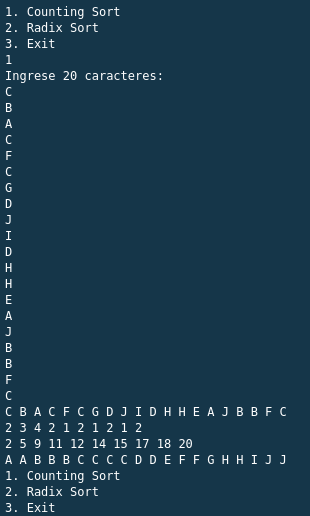
\includegraphics[scale = 1]{images/E12.png}
				\caption*{Ejercicio 1: countingSort() ejecutandose}
			\end{figure}
			
			\begin{figure}[H]
				\centering
				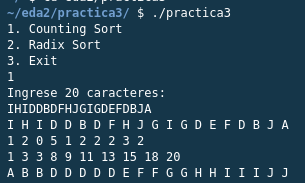
\includegraphics[scale = 1]{images/E11.png}
				\caption*{Ejercicio 1: countingSort() ejecutandose}
			\end{figure}	 
		
		\subsection{Ejercicio 2: Radix Sort}
		
			Programar el algoritmo de \emph{radixSort()} fue muy entretenido por la forma en que este ordena los elementos y cual es el proceso que usa para que todos ellos queden ordenados en forma ascendente.\\
			
			Este ejercicio se hizo tomando en cuenta que se ingresarian al menos 1 secuencia de 15 elementos de enteros cuyo rango seria desde 1111 hasta 4444 usando unicamente los digitos 1,2,3 y 4 para cada uno de ellos, lo que nos da un total de $4^4$ o 256 opciones diferentes para ingresar como elementos a este algoritmo o si repetimos elementos, entonces puede existir una infinidad.\\
			
			Una de las caracteristas de \emph{radixSort()} asi mismo, es que (al menos esta version en particular) no usa funciones alternativas para hacer el trabajo, sino que todo se declara dentro de la propia funcion.\\
			
			En los siguientes incisos, describiremos la forma en que este algoritmo funciona en este programa.
		
			\subsubsection{optionTwo()}
			
				Para comenzar a preparar el terreno para \emph{radixSort()} se comienza por ingresar a funcion la \emph{optionTwo()} cuando se escoje la opcion 2 del menu principal.
				
				Ya dentro de la funcion, declaramos una variable entera \textbf{size} que servira para ingresar la longitud del arreglo que el usuario desee crear y se imprime una leyenda solicitando que el usuario ingrese una cantidad minima de datos a ingresar que sean de al menos 15.
				
				Despues de esto, se escanea el dato ingresado dentro de un \emph{while-loop} que no se rompe sino hasta que el usuario ingresa un valor mayor o igual a 15 y cuando esto sucede se procede a imprimir otro mensaje en pantalla que solicita ingresar los elementos en funcion del tamano solicitado anteriormente. Una vez que se obtienen todos los elementos, se imprime el arreglo y se procede a ingresar a la funcion que contiene el algoritmo \emph{radixSort()}.			
			
			\subsubsection{radixSort()}
			
				La funcion \emph{radixSort()} usa dos argumentos que son, un arreglo de numeros enteros \textbf{arr} que es donde se encuentran los datos a ordenar y el tamano de tal arreglo que ya fue proporcionado por el usuario.\\
				
				La funcion \emph{radixSort()} que yo programe inicia con una variable entera \textbf{last} que se inicializa en 4 y que rompera terminara con el algoritmo cuando su valor sea 0.\\
				
				Despues se abre un \emph{do-while loop} que utiliza memoria dinamica para declarar los arreglos \textbf{arrOne}, \textbf{arrTwo}, \textbf{arrThree} y \textbf{arrFour} con un tamano de 4 bytes cada uno.\\
				
				Asi mismo se declaran 5 variables enteras que son \textbf{one}, \textbf{two}, \textbf{three}, \textbf{four} y \textbf{digit} que se inicialzan en 0 cada una.\\
				
				Asi, se comienza un \emph{for-loop} que va desde 0 hasta \textbf{size} y se ingresa a un \emph{switch} que utiliza a \textbf{last} como argumento y contiene 4 casos.\\
				
				La variable \textbf{last} existe para que en este \emph{switch} tome el digito correspondiente a cada elemento del arreglo, por lo que al valer 4 inicialmente, significa que tomara las unidades de las cifras a ordenar, cuando valga 3 tomara el digito de las decenas, 2 el de las centenas y 1 el de los miles.\\
				
				Asi cada caso dentro del \emph{switch} corresponde a la forma en que lograra esto y en el caso 4 lo unico que hara para obtener las unidades de la cifra sera obtener el \textbf{\% 10} de la cifra que proporcionara el primer digito. Para obtener el segundo digito en el momento en que \textbf{last} valga 3, entonces calculara el \textbf{\% 100} que proporcionara los ultimos dos digitos del numero (decenas y unidades), dividira entre 10 lo que dara un numero flotante (con decimal) y al final se hara un \emph{casting} a variable entera que nos proporcionara unicamente la cifra entera del numero flotante y asi obtendremos el digito para las decenas.\\
				
				El mismo proceso para las centenas pero en este caso el modulo se calcula sobre \textbf{1000} y la division sobre \textbf{100}.\\
				
				Para el caso de los miles, unicamente se divide el elemento entre \textbf{1000} y se obtiene la parte entera de la misma forma.\\
				
				El digito obtenido en el proceso se deposita en la variable \textbf{digit},\\
				
				Despues la variable \textbf{digit} se deposita en un segundo \emph{switch} que provee de acceso a cada uno de los arreglos dinamicos creados.\\
				
				Dependiendo del numero que \textbf{digit} vaya acarreando, ingresa al arreglo correspendiente. Si \textbf{digit} vale 1, entonces ingresa al area de \textbf{arrOne}, si vale 2 al area de \textbf{arrTwo} y asi dependiendo del caso.\\
				
				En el momento en que se ingresa a cualquier caso, se encuentra la variable entera correspondiente a cada uno \textbf{one, two, three o four} y se aumenta el valor de la variable correspondiente al momento de ingresar, inmediatamente despues, el arreglo pertinente \emph{resizes} (se hace de un nuevo tamano) con la ayuda de \emph{realloc()} que se multiplica por el valor que tenga la variable y se procede a depositar a la cifra correspondiente en el arreglo en el indice de la variable entera menos 1.\\
				
				Esto sucede hasta que el \emph{for-loop} inicial itera sobre todos los elementos del arreglo a ordenar y por lo tanto, deposita cada uno de los elementos en los arreglos correspondientes al digito con el que se este trabajando.\\
				
				Despues el programa ingresa a una serie de \emph{loops} que estan destinados a reacomodar todos los elementos en su arreglo original \textbf{arr} y esto sucede por medio de los valores en las variables enteras \textbf{one}, \textbf{two}, \textbf{three} y \textbf{four}.\\
				
				El primer \emph{loop} comienza en 0 hasta menos de \textbf{one} para extraer todos los elementos de \textbf{arrOne}, una vez que finaliza, ingresa al segundo \emph{loop} pero ahora este comienza desde el valor en \textbf{one} hasta el valor de \textbf{one} + \textbf{two}, pero al momento de tomar el elemento del arreglo \textbf{arrTwo} se hace desde el indice \textbf{i - (one + two)} que da el valor \textbf{0} y despues \textbf{1}, \textbf{2} y asi sucesivamente mientras va progresando el \emph{loop}. De esta forma se pueden obtener los elementos desde el indice 0 en el arreglo temporal, pero depositarlos en el indice correspondiente del arreglo original y que no se sobrescriban.\\
				
				Esto sucede a traves de otros 2 \emph{loops} hasta que terminan de iterar.\\
				
				Acto seguido se resta 1 a \textbf{last} y se procede a usar la funcion \emph{free()} para liberar la memoria de cada uno de los arreglos creados y por ultimo se imprime el arreglo con el nuevo orden numerico como la practica lo requiere.\\
				
				Asi el proceso se repite hasta que \textbf{last} es igual a 0 y cuando llega a este valor, significa que ya ha iterado sobre los 4 digitos que componen los numeros y el arreglo esta ordenado.\\
				
				Por ultimo se imprime el arreglo ordenado y se sale de la funcion.
				
			\subsubsection{Ejecucion}
			
			En la siguiente captura se muestra como se ejecuta \emph{radixSort()} con una serie de 15 cifras que no estan ordenadas.\\
			
			Se imprime cada arreglo modificado desde el originalmente no esta ordenado, hasta el que ya contiene todos los elementos en orden.
			
			\begin{figure}[H]
				\centering
				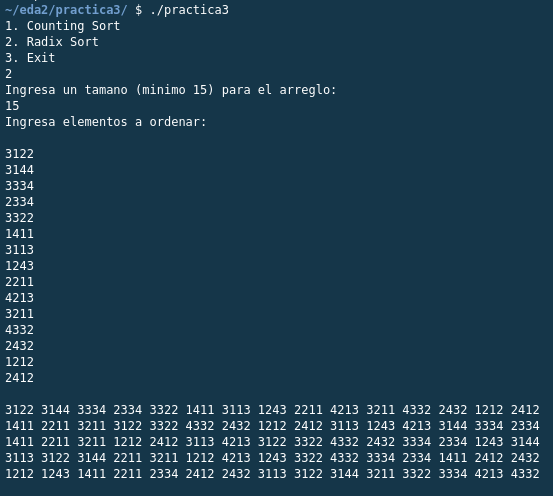
\includegraphics[scale = 0.8]{images/e3.png}
				\caption*{Ejercicio 3: Funcionamiento radixSort()}
			\end{figure}
		
		\newpage		
	
	\section{Conclusion}
	
	Algo que me gusto mucho de esta practica fue el hecho de que pude programar las funciones de los algoritmos y uno de ellos de tal forma que no tuve que buscar mucho sobre su funcionamiento en codigo como tal, sino desde el ejemplo de la prueba de escritorio en los videos me pude imaginar como seria el funcionamiento (principalmente de Radix) y a partir de ahi comence a idear una forma de programar todo el sistema para que el algoritmo pudiera resultar en algo que proporcionara una respuesta correcta.\\
	
	Probablemente esta version de Radix no sea la aceptada o correcta pues tiene en general muchos \emph{bugs} ya que fue hecha pensando en una prueba especifica de acuerdo a la practica, pero no esta hecha "a prueba de balas" aun.\\
	
	Estuve pensando en crear mi propio algoritmo de ordenamiento, pero desafortunadamente me di cuenta que ya fue inventado. Originalmente pense que se parecia mucho a \emph{Counting Sort} pero despues vi que el que es practicamente lo mismo que lo que yo pense se llama \emph{Bucket/Bin Sort}, pero algo que me he dado cuenta es que uno de los problemas es que el arreglo en el que inicialmente se implementa la informacion es estatico, cuando este deberia de ser dinamico, de tal forma que al momento que eliminas informacion del arreglo original, creas otro nodo en el arreglo ordenado y asi la complejidad espacial es constante y la temporal puede llegar a ser lineal, pero el problema es la forma en la que los archivos se ingresan primeramente.\\
	
	Esa idea se me ocurrio cuando vi el video de un hombre que ordenaba frutas pasandolas por un puente de tubos que se va cerrando y de esa manera van las frutas cayendo automaticamente en funcion de su tamano.\\
	
	Si se pudiera implementar un sistema de ordenamiento asi seria muy eficiente.\\
	
	Me parece asi, que se cumplen los objetivos de la clase sobre implementacion de estos algoritmos y el conocimiento de estos.\\
	
	Gracias por leer mi practica!
	
	\begin{figure}[H]
		\centering
		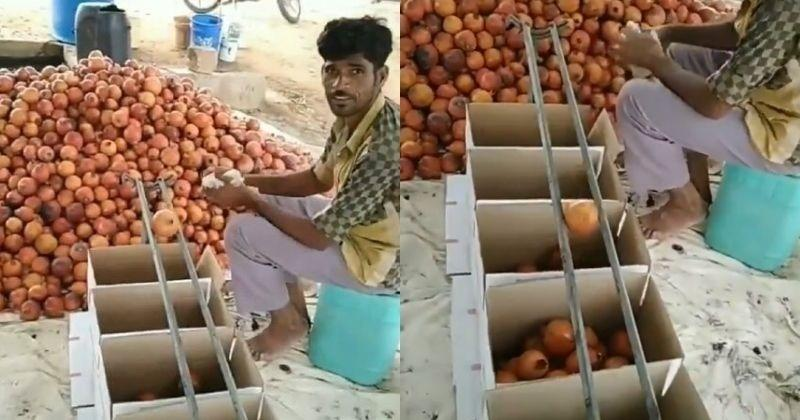
\includegraphics[scale = 0.5]{images/fruits.jpg}
		\caption*{Hombre ordenando frutas por medio de un puente de acuerdo a su tamano}		
	\end{figure}
	
	
	
	
	
	
\end{document}	
